\section{Sistema Pipeline}
Una architettura pipeline è una tipologia di soluzione che viene implementata internamente nei processori per permettere l'esecuzione parallela di più istruzioni.
Per comprendere meglio cosa si intende per esecuzione parallela di più istruzioni, andiamo a considerare la strutturazione interna del flusso di esecuzione di una normale istruzione. L'esecuzione si divide nelle seguenti fasi (visualizzabili anche alla figura [\ref{img:pipe}]):
\begin{itemize}
    \item \textbf{Istruction Fetch (IF)}: Ovvero il prelievo dell'istruzione dalla memoria
    \item \textbf{Decode (DEC)}: Decodifica ed interpretazione dell'istruzione
    \item \textbf{Execute (EX)}: Esecuzione effettiva dell'istruzione
    \item \textbf{Memory write (MW)}: Effettuo il prelievo dei dati all'interno della memoria
    \item \textbf{Register write (RW)}: Inserisco i dati che mi interessano dai registri, in memoria 
\end{itemize}

\begin{figure}
    \centering
    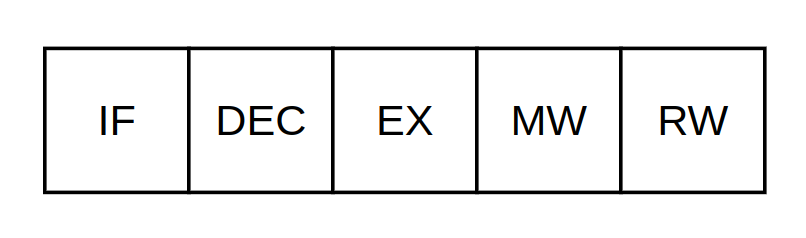
\includegraphics[width=.5\textwidth]{img/Pipeline.png}
    \caption{Architettura classica pipeline (ordine di esecuzione fasi)}\label{img:pipe}
\end{figure}

Definito il flusso di esecuzione di un istruzione, l'architettura pipeline cerca di eseguire le fasi di un istruzione in maniera del tutto separata, in modo da poter eseguire più fasi di istruzioni differenti. Per capire meglio questo concetto facciamo un esempio:
Devo eseguire un programma che ha 5 istruzioni, allora parto con l'esecuzione della prima fase, che preleverà l'istruzione i1, una volta prelevata, l'istruzione i1 passa alla fase di decode, mente, allo stesso istante, viene caricata l'istruzione i2 (quindi viene effettuata la Istruction Fetch dell'istruzione successiva mentre la prima fa la decode). Se notiamo, ed eseguiamo tale procedura per tutte le fasi noteremo che ad ogni impulso di clock (a regime), il processore darà un risultato, quindi non ci sarà bisogno di eseguire tutte le istruzioni 1 per volta, poichè la suddivisione delle fasi ne permette un esecuzione "parallela" (o meglio dire pipeline).

Per far si di isolare l'esecuzione delle varie fasi, tra i vari blocchetti saranno presenti dei registri, che permettono di conservare lo stato su cui una determinata fase sta lavorando (come le architetture pipeline in elettronica [\ref{img:pipe-reg}]). 

\begin{figure}
    \centering
    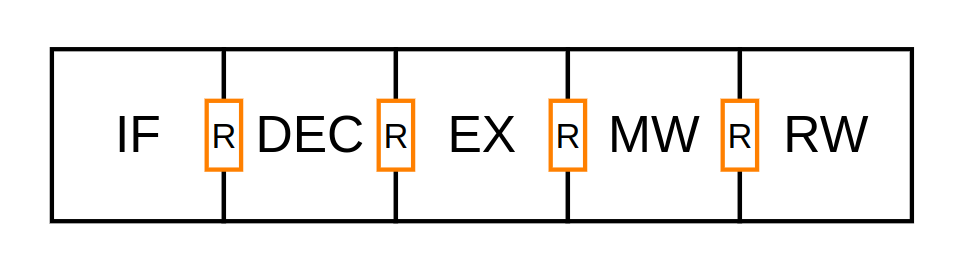
\includegraphics[width=.5\textwidth]{img/Pipe-reg.png}
    \caption{Architettura classica pipeline con registri}\label{img:pipe-reg}
\end{figure}

Un architettura di questo tipo, però, richiede una serie di ipotesi, ovvero:
\begin{itemize}
    \item Divisione di parte dati e parte istruzioni (altrimenti dovrei gestire anche dei conflitti tra l'istruction fetch e la register/memory write)
    \item Le memorie devono avere degli accessi molto veloci
    \item Le operazioni artimetico-logiche devono essere effettuate prevalentemente tra i registri interni del processore
    \item Le istruzioni devono avere tutte lunghezza fissa
\end{itemize}

Guardando le ipotesi possiamo capire che alcune tipologie di operazioni, che solitamente effettuevamo sul processore motorola, ora dovranno essere scompattate in varie operazioni. Un esempio classico è il comando \lstinline|ADD VAR,D1|, che utilizzava l'indirizzamento diretto per il prelievo dell'operando dalla memoria. In questo caso, però, l'indirizzamento diretto non è possibile, poichè si andrebbe ad invalidare un'ipotesi, ovvero, la lunghezza fissa dell'istruzione (che dovrebbe poi contenere l'indirizzo di memoria). Pertanto non sono previsti tutti i registri di memoria.

Per comprendere meglio la problematica, consideriamo di avere un prelievo dalla memoria con un architettura a 16-bit, ma con il memory address ed il memory buffer a 32-bit. Pertanto il seguente comando non sarebbe possibile: \lstinline|MOVE VAR,D0|; poichè richiederebbe il prelievo dell'indirizzo di memoria da 32-bit dalla memoria, ma per effettuare tale operazione, avendo solo 16 bit, avrei bisogno di due istruzioni che caricano, una i primi 16-bit e l'altra i restanti 16. Tale suddivisione, però non viene fatta dal programmatore, ma dal compilatore. Ci sono varie istruzioni che sono come la MOVE, tali istruzioni sono dette pseudo-istruzioni, poichè il compilatore andrà a suddividerle in più operazioni differenti al fine di raggiungere il risultato desiderato.

Questa cosa ci permette di capire, a questo punto, la suddivisione tra architettura di tipo CISC e architetture di tipo RISC. Le architetture di tipo CISC permettono l'esecuzione di istruzioni che sono più articolate, ma a costo di una complessità architetturale maggiore, mentre nelle architetture RISC, data la semplicità dell'architettura, le tipologie di operazioni che si possono effettuare sono ridotte ma più veloci.

\subsection{Modelli di sistemi pipeline}
Il sistema pipeline, dato il suo sistema di funzionamento, può introdurre varie tipologie di problematiche. Negli anni si sono sviluppate varie tipologie di soluzioni differenti.
Le principali architetture con cui si va a contatto al giorno d'oggi sono:
\begin{itemize}
    \item \textbf{MIPS}: Tipologia di ISA sviluppata da Patterson che poi ha venduto, per cui ora la sua implemetazione è proprietaria
    \item \textbf{RISC-V}: Tipologia di ISA molto simile al MIPS, ma open-source
    \item \textbf{ARM}: Tipologia di ISA proprietaria, utilizzatissima in svariati amiti (particolarmente in quello industriale), la cui implementazione è proprietaria
\end{itemize}

Nel caso particolare di questo corso, andremo a vedere il funzionamento del RISC-V facendo riferimento sempre al MIPS, per cui saranno queste le due tipologie di architetture che si andranno ad approfondire.

Le principali problematiche che bisogna affrontare all'interno di un architettura pipeline sono le seguenti:
\begin{itemize}
    \item \textbf{Interruzioni}: Quando bisogna gestire un interruzione la gestione dell'architettura pipe si complica, poichè bisogna capire chi ha interrotto e bisogna salvare lo stato di tutte le istruzioni che stanno eseguendo, che risulta una cosa molto onerosa e complicata
    \item \textbf{Concorrenza sui registi}: Se due istruzioni, devono utilizzare un informazione presente nello stesso registro ad esempio: R1 = R2+R3; R0=R1+R4;  Notiamo che per eseguire la seconda istruzione vi è bisogno del completamento della prima, ma il risultato effettivo viene scritto solo alla fine del ciclo, per cui si potrebbe incorrere in vari errori
    \item \textbf{Salti}: Quando devo effettuare un salto, se considero il caso condizionato, non so a quale ramo andrò a saltare, è quindi più complicato capire quale sarà l'istruzione successiva da eseguire
    \item \textbf{Gestione delle pipe multiple}: ho molteplici pipe di esecuzione, che quindi richiede una loro gestione per prevenire eventuali conflitti
\end{itemize}

Una delle problematiche che maggiormente incide è quella riguardante il salto, poichè, dato che non conosco quale sia l'istruzione successiva, vado a bloccare la pipe appena noto che ho un'istruzione di salto, ed appena è verificata la condizione, vado a prelevare tale istruzione dalla memoria. Però questa soluzione risulta molto inefficiente, poichè introduce dei periodi in cui la pipe rimane in stallo. Difatti, una soluzione che è stata trovata è quella della branch prediction, per cui vado a processare le istruzioni successive, cercando di prevedere quale sarà il branch da eseguire, solo nel caso in cui mi accorgo che sto sbagliando vado ad effettuare il blocco della pipe, altrimenti continuo con la normale esecuzione del programma.

